% Copyright 2004 by Till Tantau <tantau@users.sourceforge.net>.
%
% In principle, this file can be redistributed and/or modified under
% the terms of the GNU Public License, version 2.
%
% However, this file is supposed to be a template to be modified
% for your own needs. For this reason, if you use this file as a
% template and not specifically distribute it as part of a another
% package/program, I grant the extra permission to freely copy and
% modify this file as you see fit and even to delete this copyright
% notice. 

\documentclass[10pt]{beamer}
% Replace the \documentclass declaration above
% with the following two lines to typeset your 
% lecture notes as a handout:
%\documentclass{article}
%\usepackage{beamerarticle}


% There are many different themes available for Beamer. A comprehensive
% list with examples is given here:
% http://deic.uab.es/~iblanes/beamer_gallery/index_by_theme.html
% You can uncomment the themes below if you would like to use a different
% one:
%\usetheme{AnnArbor}
%\usetheme{Antibes}
%\usetheme{Bergen}
%\usetheme{Berkeley}
%\usetheme{Berlin}
%\usetheme{Boadilla}
%\usetheme{boxes}
%\usetheme{CambridgeUS}
%\usetheme{Copenhagen}
%\usetheme{Darmstadt}
%\usetheme{default}
%\usetheme{Frankfurt}
\usetheme{Goettingen}
%\usetheme{Hannover}
%\usetheme{Ilmenau}
%\usetheme{JuanLesPins}
%\usetheme{Luebeck}
%\usetheme{Madrid}
%\usetheme{Malmoe}
%\usetheme{Marburg}
%\usetheme{Montpellier}
%\usetheme{PaloAlto}
%\usetheme{Pittsburgh}
%\usetheme{Rochester}
%\usetheme{Singapore}
%\usetheme{Szeged}
%\usetheme{Warsaw}

\title{Bregman divergence optimization approaches for Logistic Regression}
\author{Ragib Zaman}


\date{28th of November, 2018}
% - Either use conference name or its abbreviation.
% - Not really informative to the audience, more for people (including
%   yourself) who are reading the slides online

\subject{Theoretical Computer Science}

% Let's get started
\begin{document}

\begin{frame}
  \titlepage
\end{frame}

\begin{frame}{Outline}
  \tableofcontents
  % You might wish to add the option [pausesections]
\end{frame}

% Section and subsections will appear in the presentation overview
% and table of contents.
\section{Background}

\subsection{Bregman Divergences}

\begin{frame}{Definition - Bregman Divergence}
Let $F: \Delta \to \mathbb{R}$ be a strictly convex function, continuously differentiable on a closed convex set $\Delta\subseteq \mathbb{R}^m.$ The Bregman Divergence generated by $F$ is a function $B_F : \Delta \times \Delta \to \mathbb{R}$ defined by $$ B_F(p,q) = F(p) - F(q) - \langle \nabla F(q), p-q \rangle$$ 

\begin{center}
 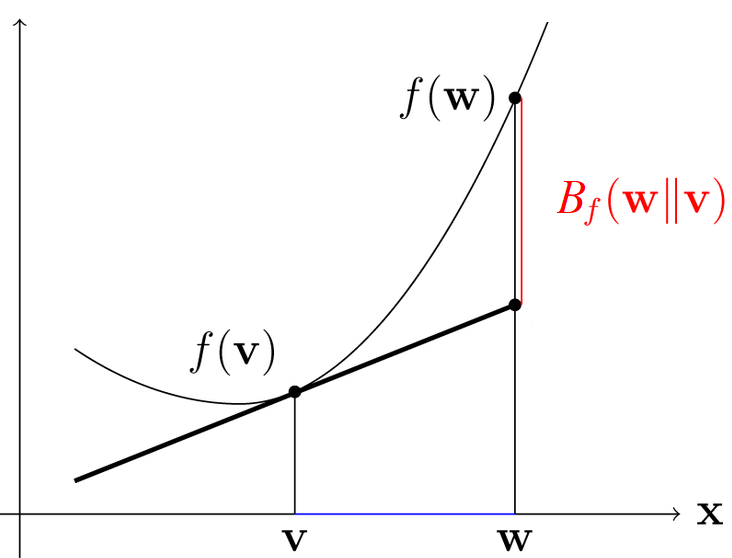
\includegraphics[scale=0.3,keepaspectratio=true]{./entropy-16-06338f2-1024.png}
 % entropy-16-06338f2-1024.png: 0x0 pixel, 0dpi, nanxnan cm, bb=
\end{center}
\end{frame}

\begin{frame}{Examples}
\begin{itemize}
 \item Squared Mahalanobis Distance
 \\
 Let $F:\mathbb{R}^m \to \mathbb{R}, x \mapsto x^TQx,$ where $Q$ is a positive definite matrix. Then $B_F(p,q) = (p-q)^T Q (p-q).$ When $Q = I_m,$ this is the squared Euclidean distance.
 
 \item Kullback-Leibler Divergence aka Relative Entropy 
 \\
 Let $F:(\mathbb{R}_{>0})^m \to \mathbb{R}, x \mapsto \sum_{i=1}^m x_i \log x_i.$ Then $$B_F(p,q) = \sum_{i=1}^m  \left( p_i \log\left(\frac{p_i}{q_i}\right) -p_i + q_i\right)$$ 
\end{itemize}

\end{frame}

\begin{frame}{Properties}
 \begin{itemize}
  \item Non-negativity: $B_F(p,q)\geq 0$ for all $p,q.$
  \item Convexity: $B_F(p,q)$ is convex in its first argument.
  \item 'Linearity': For $\alpha, \beta>0$ we have $B_{\alpha F_1 + \beta F_2}(p,q) = \alpha B_{F_1}(p,q) + \beta B_{F_2}(p,q).$
  \item Duality: Let $F^*(y) = \sup_{x\in \Delta} ( \langle x, y \rangle - F(x) )$ be the convex conjugate of $F.$ Then $$ B_{F^*}(\nabla F(p), \nabla F(q)) = B_F(p,q).$$
  \item Gradient: $\nabla_p B_F(p,q) = \nabla F(p) - \nabla F(q).$
  
 \end{itemize}

\end{frame}

\begin{frame}{Properties - Mean as Minimizer}
 \begin{Theorem}
  Suppose $P$ is a random variable taking values in $\Delta$ with distribution $\mathcal{D}.$ Then $\mathbb{E}_{P \sim \mathcal{D}}[ B_F(P,q)]$ is minimized at $q = \mathbb{E}_{\mathcal{D}}[P].$
 \end{Theorem}

 \begin{Theorem}(Banerjee et al, 2005)
  Suppose $\Delta\subseteq \mathbb{R}^m $ is a closed convex set and $d: \Delta \times \Delta \to \mathbb{R}$ is a continuously differentiable positive definite function. If $q=\mathbb{E}[P]$ is the unique minimizer of $\mathbb{E}[d(P,q)]$ for all random variables $P$ taking values in $\Delta,$ there exists a strictly convex differentiable function $F:\Delta\to\mathbb{R}$ such that $d = B_F.$
 \end{Theorem}
\end{frame}


\subsection{Logistic Regression}

% You can reveal the parts of a slide one at a time
% with the \pause command:
\begin{frame}{Logistic Regression}
Suppose we have $m$ samples of data $x_1,\ldots, x_m,$ where each $x_i\in \mathbb{R}^n$ and has a corresponding label $y_i \in \{\pm 1\}.$ Logistic Regression seeks to model the log odds-ratio by an affine function: 

$$ \log \left( \frac{ p(y_i= +1 \ | \ x_i)}{ p(y_i= -1 \ | \ x_i)} \right) = \lambda_0 + \sum_{j=1}^n \lambda_j x_{ij} := f_{\lambda}(x_i).$$ 
Indeed, Theorem 1 from (Banerjee, 2007) shows that the log odds-ratio is indeed affine if the class conditional distributions $p(x \ | \ y=+1), p(x \ | \ y=-1)$ belong to any fixed exponential family. 

\end{frame}

\begin{frame}{Logistic Regression}
 Rearranging: $$p(y_i = +1 \ | \ x) = \frac{1}{1+\exp(-f_{\lambda}(x_i))}.$$
 $$p(y_i = -1 \ | \ x) = \frac{1}{1+\exp(f_{\lambda}(x_i))}.$$
 Maxmimizing Likelihood is equivalent to minimizing the log-loss:
 $$\sum_{i=1}^m \log(1+ \exp( -y_i f_{\lambda}(x_i))$$
 This is a smooth convex function of $\lambda,$ so standard methods such as Gradient Descent and Newton's method can be applied to find $\lambda$ which minimizes the log-loss. 
\end{frame}



\section{Bregman Divergence Optimization}

\begin{frame}{Bregman Divergence Optimization}
A natural optimization problem to consider is to find the Bregman projection of a vector $q_0 \in \Delta \subseteq \mathbb{R}^m$ onto a linear subspace. Rephrased, we wish to find the $p\in \Delta$ which has least Bregman divergence to $q_0$ and satisfies some linear equality constraints. \
\newline \\
Let $\mathcal{P} = \{ p \in \Delta \ | \ p^TM = \tilde{p}^TM\}$ be the set of points satisfying the constraints, where $M$ is some $m\times n$ matrices and $\tilde{p}\in \Delta.$ \
\newline \\
Goal: Find $$\arg \min_{p\in \mathcal{P}} B_F(p, q_0).$$
\end{frame}

\begin{frame}{Bregman Divergence Optimization}
Goal: Find $$\arg \min_{p\in \mathcal{P}} B_F(p, q_0)$$ where $\mathcal{P} = \{ p \in \Delta \ | \ p^TM = \tilde{p}^TM\}.$  \
\newline \\
Idea: Define the function $\mathcal{L}_F : \Delta \times \mathbb{R}^m \to \Delta$ by $\mathcal{L}_F(q,v) = (\nabla F)^{-1}( \nabla F(q) -v).$ Let $\mathcal{Q} := \{ \mathcal{L}_F(q_0, M\lambda) \ | \lambda \in \mathbb{R}^n \} \subseteq \Delta.$ \
\newline \\
Lagrangian: $K(p,\lambda) = B_F(p,q_0) + (p^TM - \tilde{p}^TM)\lambda.$
$\nabla_p K(p,\lambda) = 0: \nabla F(p) = \nabla F(q_0) - M\lambda$ so  $p = \mathcal{L}_F(q_0, M\lambda)\in \mathcal{Q}.$\\
$\nabla_{\lambda} K(p,\lambda)= 0 : p \in \mathcal{P}.$\
\newline \\
$K(\mathcal{L}_F(q_0, M\lambda), \lambda) = B_F(\tilde{p}, q_0) - B_F(\tilde{p}, \mathcal{L}_F(q_0, M\lambda)),$ so dual to original goal is to minimize $B_F(\tilde{p}, q)$ over $q\in \mathcal{Q},$ and both problems are solved if we find a point $q_* \in \mathcal{P}\cap \mathcal{Q}.$ 
\end{frame}

\begin{frame}{Bregman Divergence Optimization}
\begin{Theorem} (Lafferty, Della Pietra, Della Pietra)\\
 For a large class of functions $F,$ there exists a unique $q_*\in \Delta$ satisfying:\\
 1) $q_* \in \mathcal{P} \cap \bar{\mathcal{Q}}.$\\
 2) $q_* = \arg \min_{q\in \bar{\mathcal{Q}}} B_F (\tilde{p}, q).$\\
 3) $q_* = \arg \min_{p\in \mathcal{P}} B_F(p, q_0).$\\
 Further, any of these properties determines $q_*$ uniquely. 
\end{Theorem}
 We will express the problem of minimizing the log-loss of Logistic Regression as a problem of type 2.
\end{frame}

\begin{frame}{Logistic Regression Revisited}

Let $\Delta = [0,1]^m.$ Let $\tilde{p} = \mathbf{0}, q_0 = (1/2) \mathbf{1},$ and $M_{ij} = y_i x_{ij}.$ Let $F(p) = \sum_{i=1}^m \left( p_i \log p_i + (1-p_i) \log(1-p_i) \right).$ Then we have $ \mathcal{L}_F(q,v)_i = \frac{q_i e^{-v_i}}{1-q_i + q_i e^{-v_i}}$ so that $$\mathcal{Q} = \bigg\{ q\in [0,1]^m \ | \ q_i = \sigma\left( \sum_{j=1}^n \lambda_j y_i x_{ij} \right), \lambda \in \mathbb{R}^n \bigg\},$$ where $\sigma(x) = 1/(1+e^x).$ We also have $$ B_F(p,q) = \sum_{i=1}^m \left( p_i \log \left( \frac{p_i}{q_i} \right) + (1-p_i) \log \left( \frac{1-p_i}{1-q_i} \right) \right)$$ so $B_F(\mathbf{0}, q) = -\sum_{i=1}^m \log(1-q_i).$ Thus, $$B_F(\mathbf{0}, \mathcal{L}_F(q_0, M\lambda)) = \sum_{i=1}^m \log\left(1+\exp\left(-y_i\sum_{j=1}^n \lambda_j x_{ij}\right) \right)$$ so minimizing log-loss is minimizing $B_F(\mathbf{0}, q)$ over $q\in \bar{\mathcal{Q}}.$ 
\end{frame}



\begin{frame}{Logistic Regression Algorithm (Collins, Schapire, Singer)}

Parameters: $\Delta = [0,1]^m,$ $q_0 = (1/2) \mathbf{1},$ and $F(p) = \sum_{i=1}^m \left( p_i \log p_i + (1-p_i) \log(1-p_i) \right).$\
\newline \\
Input: $M_{ij} = y_i x_{ij}$ where $\sum_{j=1}^n |M_{ij}| \leq 1$ for all $i.$ \
\newline \\
Output: $(\lambda_t)_{t=1,2,\ldots}$ such that $$ \lim_{t\to\infty} B_F(\mathbf{0}, \mathcal{L}_F(q_0, M\lambda_t)) = \inf_{\lambda\in\mathbb{R}^n} B_F(\mathbf{0}, \mathcal{L}_F(q_0, M\lambda)).$$ \
\newline \\
\end{frame}

\begin{frame}{Logistic Regression Algorithm (Collins, Schapire, Singer)}
 Algorithm: \ Let $\lambda_1=\mathbf{0}.$
\newline For $t=1,2,3, \ldots$ : \
\newline - \ \ \ $q_t = \mathcal{L}_F(q_0, M\lambda_t)$ \
\newline - \ \ \ For $j=1,2,\ldots, n:$ $$W^+_{t,j} = \sum_{i : \operatorname{sign}(M_{ij}) = +1 } q_{t,i} |M_{ij}|$$ $$ W^-_{t,j} = \sum_{i : \operatorname{sign}(M_{ij}) = -1 } q_{t,i} |M_{ij}|$$ $$ \delta_{t,j} = \frac{1}{2} \log \left( \frac{ W^+_{t,j}}{W^-_{t,j}} \right) $$\
\newline - \ \ \ Let $\lambda_{t+1} = \lambda_t + \delta_t.$ 
\end{frame}


% Placing a * after \section means it will not show in the
% outline or table of contents.

\begin{frame}{Extensions}
 \begin{itemize}
  \item Same framework can be applied to AdaBoost
  \item Algorithm can be extended to include Ivanov regularisation. L1 regularization handled in (Huang and Gupta, 2008). 
 \end{itemize}

\end{frame}



\section*{Summary}

\begin{frame}{Summary}
  \begin{itemize}
  \item
    Bregman divergences are fundamental in the study of convexity and its applications
  \item
    They can be used to create new optimization algorithms
  \item
   They can be used to find connections between seemingly different optimization problems
  \end{itemize}
  
\end{frame}



% All of the following is optional and typically not needed. 
\appendix
\section<presentation>*{\appendixname}
\subsection<presentation>*{References}

\begin{frame}[allowframebreaks]
  \frametitle<presentation>{References}
    
  \begin{thebibliography}{10}
    
  \beamertemplatearticlebibitems
  % Followed by interesting articles. Keep the list short. 

  \bibitem{Someone2000}
    M.~Collins, R.E.~Schapire, Y.~Singer
    \newblock Logistic Regression, AdaBoost and Bregman Distances.
    \newblock {\em Machine Learning}, 48(1/2/3).
    2002.
    
    \bibitem{Someone2000}
    T.~Huang, M.~Gupta
    \newblock Bregman distance to L1 regularized logistic regression.
    \newblock {\em International Conference on Pattern Recognition}
    2008.  
    
    \bibitem{Someone2000}
    A.~Banerjee
    \newblock An Analysis of Logistic Models:
Exponential Family Connections and Online Performance.
    \newblock {\em 2007 SIAM International Conference on Data Mining}
    2007.  
    
    \bibitem{Someone2000}
    A.~Banerjee, X.~Gou, H.~Wang
    \newblock  On the Optimality of Conditional Expectation as a Bregman Predictor.
    \newblock {\em IEEE Trans. on Information Theory} Vol 51(7)
    2005.  
    
    \bibitem{Someone2000}
    J.~Lafferty, S.~Della Pietra, V.~Della Pietra
    \newblock  Inducing Features of Random Fields.
    \newblock {\em IEEE Trans. Pattern Analysis and Machine Intelligence} Vol 19(4)
    1997.
  \end{thebibliography}
\end{frame}

\end{document}


